\section{Fine-grained Entity Typing with KENN} \label{et_with_kenn}
We saw in section \ref{entity_typing} that Fine-grained Entity Typing (FET) is a multilabel classification problem, where the goal is to assign one or more types from a type set to a mention appearing in a text. This section will present the FET datasets used for the experiments and the architecture of the adopted models.


\subsection{Datasets}
Several datasets were proposed through the years to evaluate the task of FET. Since building large annotated datasets is an expensive task, most of them are built using Distant Supervision techniques. Some state-of-the-art datasets used to evaluate FET approaches are FIGER~\cite{Ling2012FineGrainedER}, BBN~\cite{ren-etal-2016-afet}, OntoNotes~\cite{ontonotes} and Choi~\cite{choi}. While the first three datasets have tree-like structures to group types hierarchically, Choi is organized differently. It groups the types into three categories: general, fine-grained, and ultra-fine-grained. Each dataset is provided with its own type set and is split into training set and test set. While every training set is obtained through distant supervision, test sets are manually annotated for most of them.

This thesis focuses the experiments on two of the most popular datasets: FIGER and BBN. The reason behind the choice is that they have a less complex hierarchy than OntoNotes, thus allowing us to better comprehend how KENN influences the task and how to take advantage of it. Regarding Choi, it has not been considered for this work because types are not hierarchically organized.

\subsubsection{FIGER}
FIGER is one of the first FET datasets. It was presented in 2012 with Fine-Grained Entity Recognition~\cite{Ling2012FineGrainedER}. The original version of the dataset is based on a type set $T$ derived from Freebase~\cite{bollacker2008freebase} and counts a total of 112 types. The hierarchy is organized as a forest of trees with maximum depth 1, i.e., 2-level hierarchy. A summary of the type set can be found in Figure~\ref{fig:figer}.

\begin{figure}
    \centering
    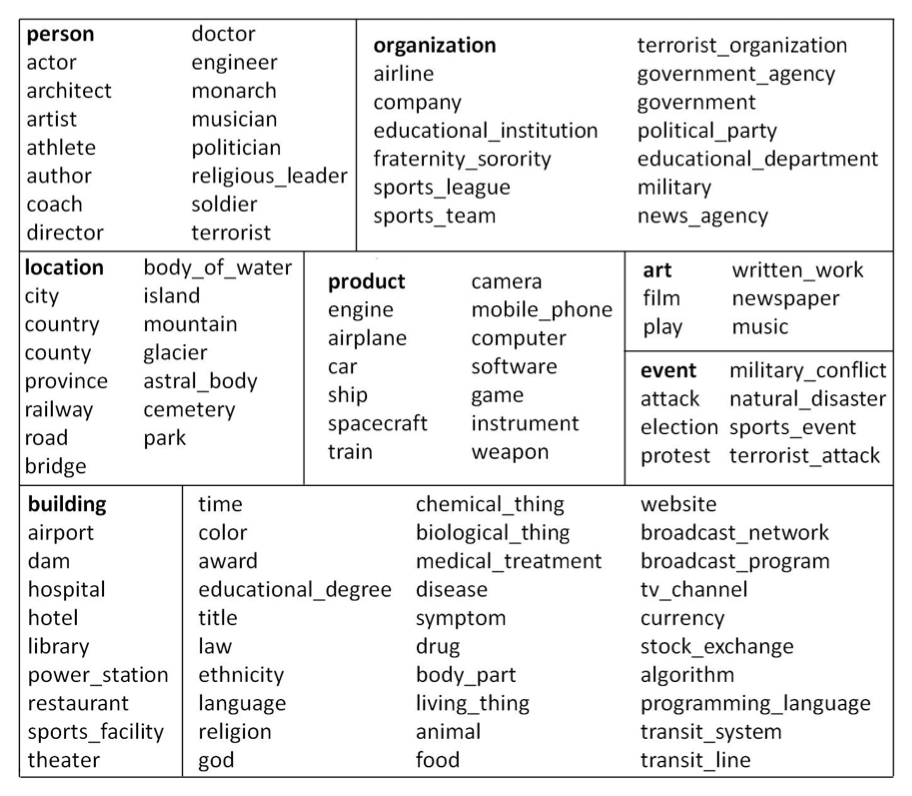
\includegraphics[width=0.7\linewidth]{figer.png}
    \caption{Type set of FIGER. Each box can be seen as a two-level tree, with the root node represented by the type in bold. The box at the bottom right is composed of uncategorized types. (Source:~\cite{Ling2012FineGrainedER})}
    \label{fig:figer}
\end{figure}

As said previously, the training set is obtained with a distant supervision technique and counts about $1.5M$ instances. The source of data that has been labeled is constituted by Wikipedia articles, where anchor links are treated as entity mentions. The annotation procedure can be summarized in three steps:
\begin{enumerate}
    \item For each sentence, detect all the linked segments $m$
    \item For each $m$, retrieve the related Wikipedia entity $e_{m}$
    \item For each $e_{m}$, obtain its types $t'_{m}$ from Freebase
    \item For each $t'_{m}$, refine the types to obtain a subset $t_{m} \subseteq t'_{m}$ such that $t_{m} \subseteq T$. The refinement is done by keeping only the ones with more than 5 ground instances and merging types that are too specific.
\end{enumerate}

The test set is composed of 434 manually annotated examples. The sentences are extracted from local newspapers, photography and veterinary magazines, and the student newspaper of the University of Washington.

Each entry of the dataset is represented following the structure of the JSON in Figure~\ref{fig:entry_bbn}. The main fields are \textit{tokens}, which contains the list of the worlds of the sentence, and \textit{mentions}. For each mention there are three subfields: \textit{start} and \textit{end} indicate the index of the tokens that delimits the mention, and \textit{labels} contains the true types.

\begin{figure}
    \centering
    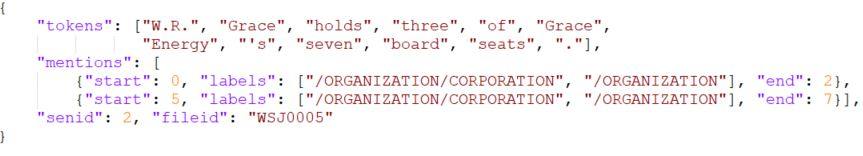
\includegraphics[width=1\linewidth]{figures/entry_bbn.JPG}
    \caption{Structure of a FIGER/BBN entry. Example taken from BBN.}
    \label{fig:entry_bbn}
\end{figure}

\subsubsection{BBN}
BBN dataset for FET made its first appearance in~\cite{ren2016noise} in 2016. The original version of this dataset comes from the BBN Pronoun Coreference and Entity Type Corpus~\cite{bbnCoreference}, composed of manually annotated Wall Street Journal articles. These articles were originally annotated using 93 types, divided into 12 named entity types, 9 nominal entity types, 7 numeric types, and 64 subtypes. However, when applying distant supervision, the authors used DBpedia Spotlight to link entities and they had to remove those BBN types that could not be mapped into Freebase types. The resulting type set counts 47 types.

The dataset is constituted by 32,739 entries. The test set has not been manually annotated. To construct it, the authors simply extracted a subset composed of the 20\% of the dataset,

An entry of the dataset is structured in the same way as FIGER (Figure~\ref{fig:entry_bbn}), so we can find the sentence as \textit{tokens} and the \textit{mentions} including \textit{start}, \textit{end} and \textit{labels} as subfields.

\subsubsection{Dataset preparation \& statistics} \label{dataset_stats}
The adopted versions of the datasets are those proposed by Ren et al. in~\cite{ren-etal-2016-afet}\footnote{https://github.com/INK-USC/AFET}. Before performing the experiments, both training sets of FIGER and BBN were refined. First of all, the duplicates (i.e., instances with the same context, mention, and types) were removed. Then, examples having the same context and different sets of mentions were merged. Each entry with more than one mention was subsequently divided into distinct entries with single mentions. Regarding FIGER, the equivalent types \texttt{/living\_thing} and \texttt{/livingthing} were unified in \texttt{/living\_thing}. Finally the sentences were split into 3 fields: \textit{left\_context\_token}, \textit{mention\_span} and \textit{right\_context\_token}. The mention types can be found in the field \textit{y\_str}. An example of an entry of the refined dataset is available in Figure~\ref{fig:entry_bbn_clean}. Since the dev sets were not provided within the original datasets, they were obtained by sampling about 1K instances of the training sets, such that single-mention examples derived from the same multi-mention example are assigned to the same set.

\begin{figure}
    \centering
    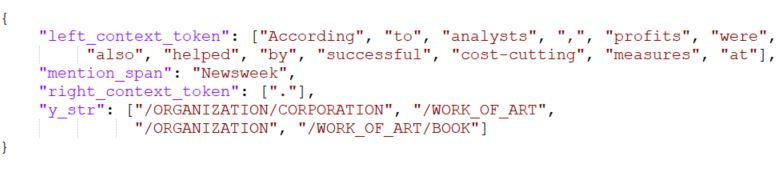
\includegraphics[width=1\linewidth]{figures/entry_bbn_clean.JPG}
    \caption{Structure of a FIGER/BBN entry after data preparation - Example taken from BBN}
    \label{fig:entry_bbn_clean}
\end{figure}

Before proceeding with the analysis of the datasets, it is helpful to point out that every sentence can contain multiple types from different branches. We will refer to this condition with the term multibranch. Furthermore, if an instance $x$ of the dataset is labeled with a type $t$ that is a subtype of $t'$, then the type set of $x$ must contain both $t$ and $t'$.

In Table~\ref{tab:dataset_stats} we can find some useful statistics about the two datasets. The fields of the table can be described as follows:
\begin{itemize}
    \item \textbf{\# ex:} number of examples of the refined version of the dataset
    \item \textbf{\% only supertype:} percentage of examples where a coarse type occurs without any of its subtypes
    \item \textbf{\% only supertype (strict):} percentage of examples where only coarse types occur
    \item \textbf{\% inter-tree:} percentage of examples where sibling types occur together
    \item \textbf{\% intra-tree:} percentage of examples where types from different trees occur together
    \item \textbf{\% intra/inter-tree:} percentage of examples where types from different branches occur together\footnote{this statistic is not equivalent to \textit{\%~inter-tree}~+~\%~intra-tree, since in the same example we could find both the situations}
    \item \textbf{\# types:} number of types of the refined version of the dataset
    \item \textbf{\# avg types:} average number of types per example
    \item \textbf{\% isolated types:} percentage of types corresponding to an isolated node\footnote{node without any parent or child} of the hierarchy
\end{itemize}

Looking at the table, it is possible to draw some considerations. In both datasets, we can observe that the multibranch examples are mostly caused by the presence of \textit{inter-tree} types. Regarding FIGER, we see that the statistics about \textit{only~supertype} are widely different between the training/dev and test sets. We have about the 21\% of cases against the 60\%, becoming 15\% against 54\% considering the \textit{strict} mode. This diversity derives from the manual annotation, where probably the types annotated through distant supervision that were too specific have been removed by the annotators. Even the statistics of \textit{intra/inter-tree} differ a lot between the training/dev and test sets. In this case, we move from the 35\% of multibranch examples to the 11\%. Again, the reason can be found in the manual annotation. Indeed, when using distant supervision techniques, a mention can be labeled with all its meanings disregarding the context. To point out how noisy is FIGER, we can also see how the \textit{\#~avg~types} statistic drastically decreases after the manual annotation.

Moving on to BBN, which does not have a manually annotated test set, the situation is quite different. First of all, we can notice that while the training/dev set counts the 22-24\% of multibranch examples, in the test set they are absent. This statistic is motivated by the fact that Ren et al. pruned these examples from the test set. For the same reason, we have no difference between the values of \textit{\%~only~supertype} and \textit{\%~only~supertype~(strict)} in the test. 

\begin{table}
\centering
\caption{Datasets statistics}
\label{tab:dataset_stats}
\resizebox{\columnwidth}{!}{\begin{tabular}{cccclll}
\hline
\multicolumn{1}{|c|}{\textbf{Dataset}} & \multicolumn{1}{c|}{\textbf{\# ex}}    & \multicolumn{1}{c|}{\textbf{\% only supertype}} & \multicolumn{1}{c|}{\textbf{\begin{tabular}[c]{@{}c@{}}\% only supertype\\ (strict)\end{tabular}}} & \multicolumn{1}{c|}{\textbf{\% inter-tree}} & \multicolumn{1}{c|}{\textbf{\% intra-tree}} & \multicolumn{1}{c|}{\textbf{\% inter/intra-tree}} \\ \hline
\multicolumn{1}{|c|}{BBN train}        & 84,492                                 & 16.0                                            & 7.64                                                                                               & \multicolumn{1}{c}{22.33}                   & \multicolumn{1}{c}{2.65}                    & \multicolumn{1}{c|}{24.09}                        \\
\multicolumn{1}{|c|}{BBN dev}          & 1,039                                  & 15.3                                            & 8.47                                                                                               & \multicolumn{1}{c}{20.69}                   & \multicolumn{1}{c}{2.31}                    & \multicolumn{1}{c|}{22.52}                        \\
\multicolumn{1}{|c|}{BBN test}         & 12,349                                 & 7.44                                            & 7.44                                                                                               & \multicolumn{1}{c}{-}                       & \multicolumn{1}{c}{-}                       & \multicolumn{1}{c|}{-}                            \\ \hline
\multicolumn{1}{|c|}{FIGER train}      & 2,676,854                              & 21.33                                           & 14.99                                                                                              & \multicolumn{1}{c}{23.63}                   & \multicolumn{1}{c}{15.38}                   & \multicolumn{1}{c|}{35.23}                        \\
\multicolumn{1}{|c|}{FIGER dev}        & 1,094                                  & 21.57                                           & 14.72                                                                                              & \multicolumn{1}{c}{25.59}                   & \multicolumn{1}{c}{14.35}                   & \multicolumn{1}{c|}{35.83}                        \\
\multicolumn{1}{|c|}{FIGER test}       & 563                                    & 60.57                                           & 54.17                                                                                              & \multicolumn{1}{c}{11.01}                   & \multicolumn{1}{c}{0.71}                    & \multicolumn{1}{c|}{11.72}                        \\ \hline
\multicolumn{1}{l}{}                   & \multicolumn{1}{l}{}                   & \multicolumn{1}{l}{}                            & \multicolumn{1}{l}{}                                                                               &                                             &                                             &                                                   \\ \cline{1-4}
\multicolumn{1}{|c|}{\textbf{Dataset}} & \multicolumn{1}{c|}{\textbf{\# types}} & \multicolumn{1}{c|}{\textbf{\# avg types}}      & \multicolumn{1}{c|}{\textbf{\% isolated types}}                                                    &                                             &                                             &                                                   \\ \cline{1-4}
\multicolumn{1}{|c|}{BBN train}        & 157,292                                & 1.86                                            & \multicolumn{1}{c|}{24.3}                                                                          &                                             &                                             &                                                   \\
\multicolumn{1}{|c|}{BBN dev}          & 1,903                                  & 1.83                                            & \multicolumn{1}{c|}{24.44}                                                                         &                                             &                                             &                                                   \\
\multicolumn{1}{|c|}{BBN test}         & 20,606                                 & 1.67                                            & \multicolumn{1}{c|}{15.4}                                                                          &                                             &                                             &                                                   \\ \cline{1-4}
\multicolumn{1}{|c|}{FIGER train}      & 6,380,532                              & 2.38                                            & \multicolumn{1}{c|}{9.21}                                                                          &                                             &                                             &                                                   \\
\multicolumn{1}{|c|}{FIGER dev}        & 2,616                                  & 2.39                                            & \multicolumn{1}{c|}{9.79}                                                                          &                                             &                                             &                                                   \\
\multicolumn{1}{|c|}{FIGER test}       & 840                                    & 1.49                                            & \multicolumn{1}{c|}{6.55}                                                                          &                                             &                                             &                                                   \\ \cline{1-4}
\end{tabular}}
\end{table}

The information about the hierarchy of each dataset are reported in Table~\ref{tab:dataset_hierarchy}. The columns of the table can be described as follows:
\begin{itemize}
    \item \textbf{\# nodes:} number of nodes of the hierarchy (i.e., cardinality of the type set)
    \item \textbf{\# levels:} maximum number of levels of a tree in the type set
    \item \textbf{\# top level:} number of root nodes with at least a child (i.e., supertypes)
    \item \textbf{\# leaves:} number of child nodes (i.e., subtypes)
    \item \textbf{\# isolated:} number of isolated nodes (i.e., neither supertypes nor subtypes)
\end{itemize}

\begin{table}
\centering
\caption{Datasets hierarchical structure}
\label{tab:dataset_hierarchy}
\begin{tabular}{|c|ccccc|}
\hline
\textbf{Dataset} & \multicolumn{1}{c|}{\textbf{\# nodes}} & \multicolumn{1}{c|}{\textbf{\# levels}} & \multicolumn{1}{c|}{\textbf{\# top level}} & \multicolumn{1}{c|}{\textbf{\# leaves}} & \textbf{\# isolated} \\ \hline
BBN              & 47                                     & 2                                       & 9                                          & 31                                      & 7                    \\ \hline
FIGER            & 128                                    & 2                                       & 22                                         & 79                                      & 27                   \\ \hline
\end{tabular}
\end{table}

\subsection{Baseline model} \label{baseline_model}
The architecture of the baseline network used in the experiments is shown in Figure~\ref{fig:et_baseline_architecture}. Starting from the input, the text is composed of three parts: left context (LC), mention (M), and right context (RC). The encoder receives a sequence in the form of \verb|[CLS]M[SEP]LC[SEP]RC|.  The example in the picture reports BERT as encoder, but any variant could be used to take its place. The versions used to perform the experiments of this thesis are BERT large\footnote{https://huggingface.co/bert-large-cased} and DistilBERT\footnote{https://huggingface.co/distilbert-base-uncased} for PyTorch\footnote{https://pytorch.org/}. In any case, the encoders are trained using the adapters with the Pfeiffer strategy. The framework used to integrate them into the models is AdapterHub\footnote{https://github.com/Adapter-Hub/adapter-transformers}. Once the encoder produces the output sequence, the encoding of the \verb|[CLS]| token is fed into a basic neural network composed of a fully connected layer and a classification layer. The fully connected layer has the same dimension as the encoder's output, the classification layer applies the sigmoid activation function to compute the probability to assign each label. Finally, there is the inference step to obtain the final predictions starting from the probabilities (more details in section~\ref{inference_rules}).

\begin{figure}[H]
    \centering
    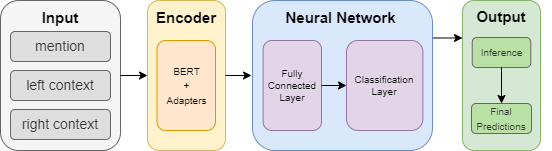
\includegraphics[width=.8\linewidth]{figures/et_baseline_architecture.png}
    \caption{Baseline model architecture}
    \label{fig:et_baseline_architecture}
\end{figure}


\subsection{KENN model} \label{kenn_model}
The architecture of the KENN-based model is designed starting from the baseline. As we can see in Figure~\ref{fig:et_kenn_architecture}, the architecture of the two models is almost the same. The only differences are the presence of KENN in the middle of the network and the KB provided to the model. The knowledge enhancement layer is placed between the fully connected layer and the classification layer. What said for the baseline model about input representation, encoders, etc. is still valid for this model.

\begin{figure}[H]
    \centering
    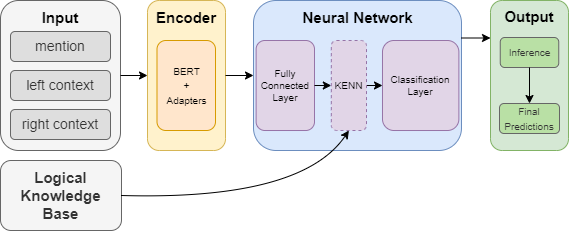
\includegraphics[width=.8\linewidth]{figures/et_kenn_architecture.png}
    \caption{KENN-based model architecture}
    \label{fig:et_kenn_architecture}
\end{figure}

Among the strategies for defining logical KB proposed in section~\ref{knowledge_generation}, the ones chosen for the experiments are the \textit{Bottom Up}, \textit{Top Down}, and \textit{Hybrid}. Other KB modes from Table~\ref{tab:kb_modes} are not taken into account since they do not apply to datasets with a 2-level hierarchy. We will not even analyze horizontal constraints since the priority has been given to the vertical ones. The number of clauses generated by the chosen KB modes are reported in Table~\ref{tab:dataset_clauses}.

\begin{table}
\centering
\caption{Datasets and number of clauses}
\label{tab:dataset_clauses}
\begin{tabular}{|c|ccc|}
\hline
\textbf{Dataset} & \multicolumn{1}{c|}{\textbf{Bottom Up}} & \multicolumn{1}{c|}{\textbf{Top Down}} & \textbf{Hybrid} \\ \hline
BBN              & 31                                      & 9                                      & 40              \\ \hline
FIGER            & 79                                      & 22                                     & 101             \\ \hline
\end{tabular}
\end{table}

Depending on the KB mode, KENN affects the predictions of the baseline network in different ways. Some statistics about the influence of the logical knowledge are available in Table~\ref{tab:dataset_stats_kenn}, which provides the following information:
\begin{itemize}
    \item \textbf{\% no clauses:} percentage of examples labeled with at least one type that does not occur in any clause (i.e. isolated type)
    \item \textbf{\% no clauses (strict):} percentage of examples labeled exclusively with types that do not occur in any clause (i.e. isolated types only)
    \item \textbf{\% inappropriate Top Down rules:} percentage of examples in which a supertype occurs without any of its subtypes; equivalent to \textit{\% only supertype} in Table~\ref{tab:dataset_stats}
    \item \textbf{\% inappropriate Top Down rules (strict):} percentage of examples in which only supertypes occur; equivalent to \textit{\% only supertype (strict)} in Table~\ref{tab:dataset_stats}
\end{itemize}
With the term \textit{``inappropriate"} used in the last two statistics, we mean that the intervention of KENN may be undesired. Contrarily to what happens in Bottom Up, the knowledge enhancement could be disadvantageous when using the Top Down mode in some cases. The reason is that a Top Down clause will always encourage the model to predict subtypes even when the ground truth contains only supertypes. Indeed, we saw in section~\ref{knowledge_generation} that while Bottom Up respects the Open World Assumption, Top Down is defined under the Closed World Assumption. About the statistics from the table, we can notice relevant differences between the train/dev and the test sets. The most evident one regards FIGER and the \textit{Top Down} statistics, where we can observe a difference of 40 percentage points.


\begin{table}
\centering
\caption{Datasets statistics on KENN's influence}
\label{tab:dataset_stats_kenn}
\resizebox{\columnwidth}{!}{\begin{tabular}{|c|cccc|}
\hline
\textbf{Dataset} & \multicolumn{1}{c|}{\textbf{\% no clauses}} & \multicolumn{1}{c|}{\textbf{\begin{tabular}[c]{@{}c@{}}\% no clauses\\ (strict)\end{tabular}}} & \multicolumn{1}{c|}{\textbf{\begin{tabular}[c]{@{}c@{}}\% inappropriate\\ Top Down rules\end{tabular}}} & \textbf{\begin{tabular}[c]{@{}c@{}}\% inappropriate\\ Top Down rules\\ (strict)\end{tabular}} \\ \hline
BBN train        & 44.74                                       & 37.01                                                                                          & 16.00                                                                                                   & 7.64                                                                                          \\
BBN dev          & 44.47                                       & 37.05                                                                                          & 15.30                                                                                                   & 8.47                                                                                          \\
BBN test         & 25.69                                       & 25.69                                                                                          & 7.44                                                                                                    & 7.44                                                                                          \\ \hline
FIGER train      & 18.06                                       & 9.85                                                                                           & 21.33                                                                                                   & 14.99                                                                                         \\
FIGER dev        & 20.02                                       & 10.79                                                                                          & 21.57                                                                                                   & 14.72                                                                                         \\
FIGER test       & 9.59                                        & 5.33                                                                                           & 60.57                                                                                                   & 54.17                                                                                         \\ \hline
\end{tabular}}
\end{table}

\subsection{Inference rules} \label{inference_rules}
The scores produced by the model can be processed through different inference rules to transform the probability of each class into a binary prediction. The most common strategy to discriminate between positive and negative predictions in classification problems is to use a threshold, but there are many alternatives that may lead to better results. The choice of the inference rule may heavily affect the evaluation of a model. Given an instance, we indicate with $Y$ the set of output values of the neural network and with $y$ the output for a specific type. The inference rules that will be used to compute the final predictions are the following:
\begin{enumerate}
    \item \textbf{Threshold:} basic inference method which simply compare the scores with the threshold
    \begin{gather*}
        pred(y) = 1 \iff score(y) > threshold
    \end{gather*}
    \item \textbf{Threshold or max:} same as \textit{threshold}'s method, but it prevents void predictions by assigning the class with maximum score when none of the scores exceeds the threshold
    \begin{gather*}
        pred(y) = 1 \iff (score(y) > threshold \vee score(y) = \max_{y_{i}\in Y}score(y_{i}))
    \end{gather*}
    This inference rule is commonly used by FET from the literature.
\end{enumerate}